\documentclass[11pt]{article}
\usepackage[sort]{natbib}
\usepackage{bm,amsmath,bbm,amsfonts,nicefrac,latexsym,amsmath,amsfonts,amsbsy,amscd,amsxtra,amsgen,amsopn,bbm,amsthm,amssymb,graphicx}
\usepackage{fancyhdr}
\usepackage[margin=1.0in]{geometry}
\usepackage[section]{placeins}
\bibliographystyle{abbrvnat}

\title{Thesis Introduction}
\author{Ewan Pinnington}

\newtheorem{theorem}{Theorem}[section]
\newtheorem*{defn}{Definition}


\begin{document}

\maketitle

\section{Notation}
List of symbols and meanings consistent throughout thesis.

\section{The global carbon cycle}

Carbon is one of the most abundant elements, making up around half of all the dry mass of living matter on Earth. The global carbon cycle describes the movement of carbon through the Earth system. In the Earth system large amounts of carbon are present in the oceans, atmosphere, land surface and crust. These stores of carbon are referred to as reservoirs or pools. The amount of carbon on Earth can be considered constant as under terrestrial conditions it is not common to have nuclear transmutation. Therefore terrestrial processes using carbon must transfer it between the global carbon pools, this is referred to as a flux.

Greenhouse gas effect of CO2 in the atmosphere, CO2 one of contributing compounds. CO2 most important human-contributed compound \citep{Falkowski291}.

Human emissions of CO2 have perturbed the global C cycle and caused a large continual increase in atmospheric CO2 levels.

\begin{figure}[ht]
    \centering
    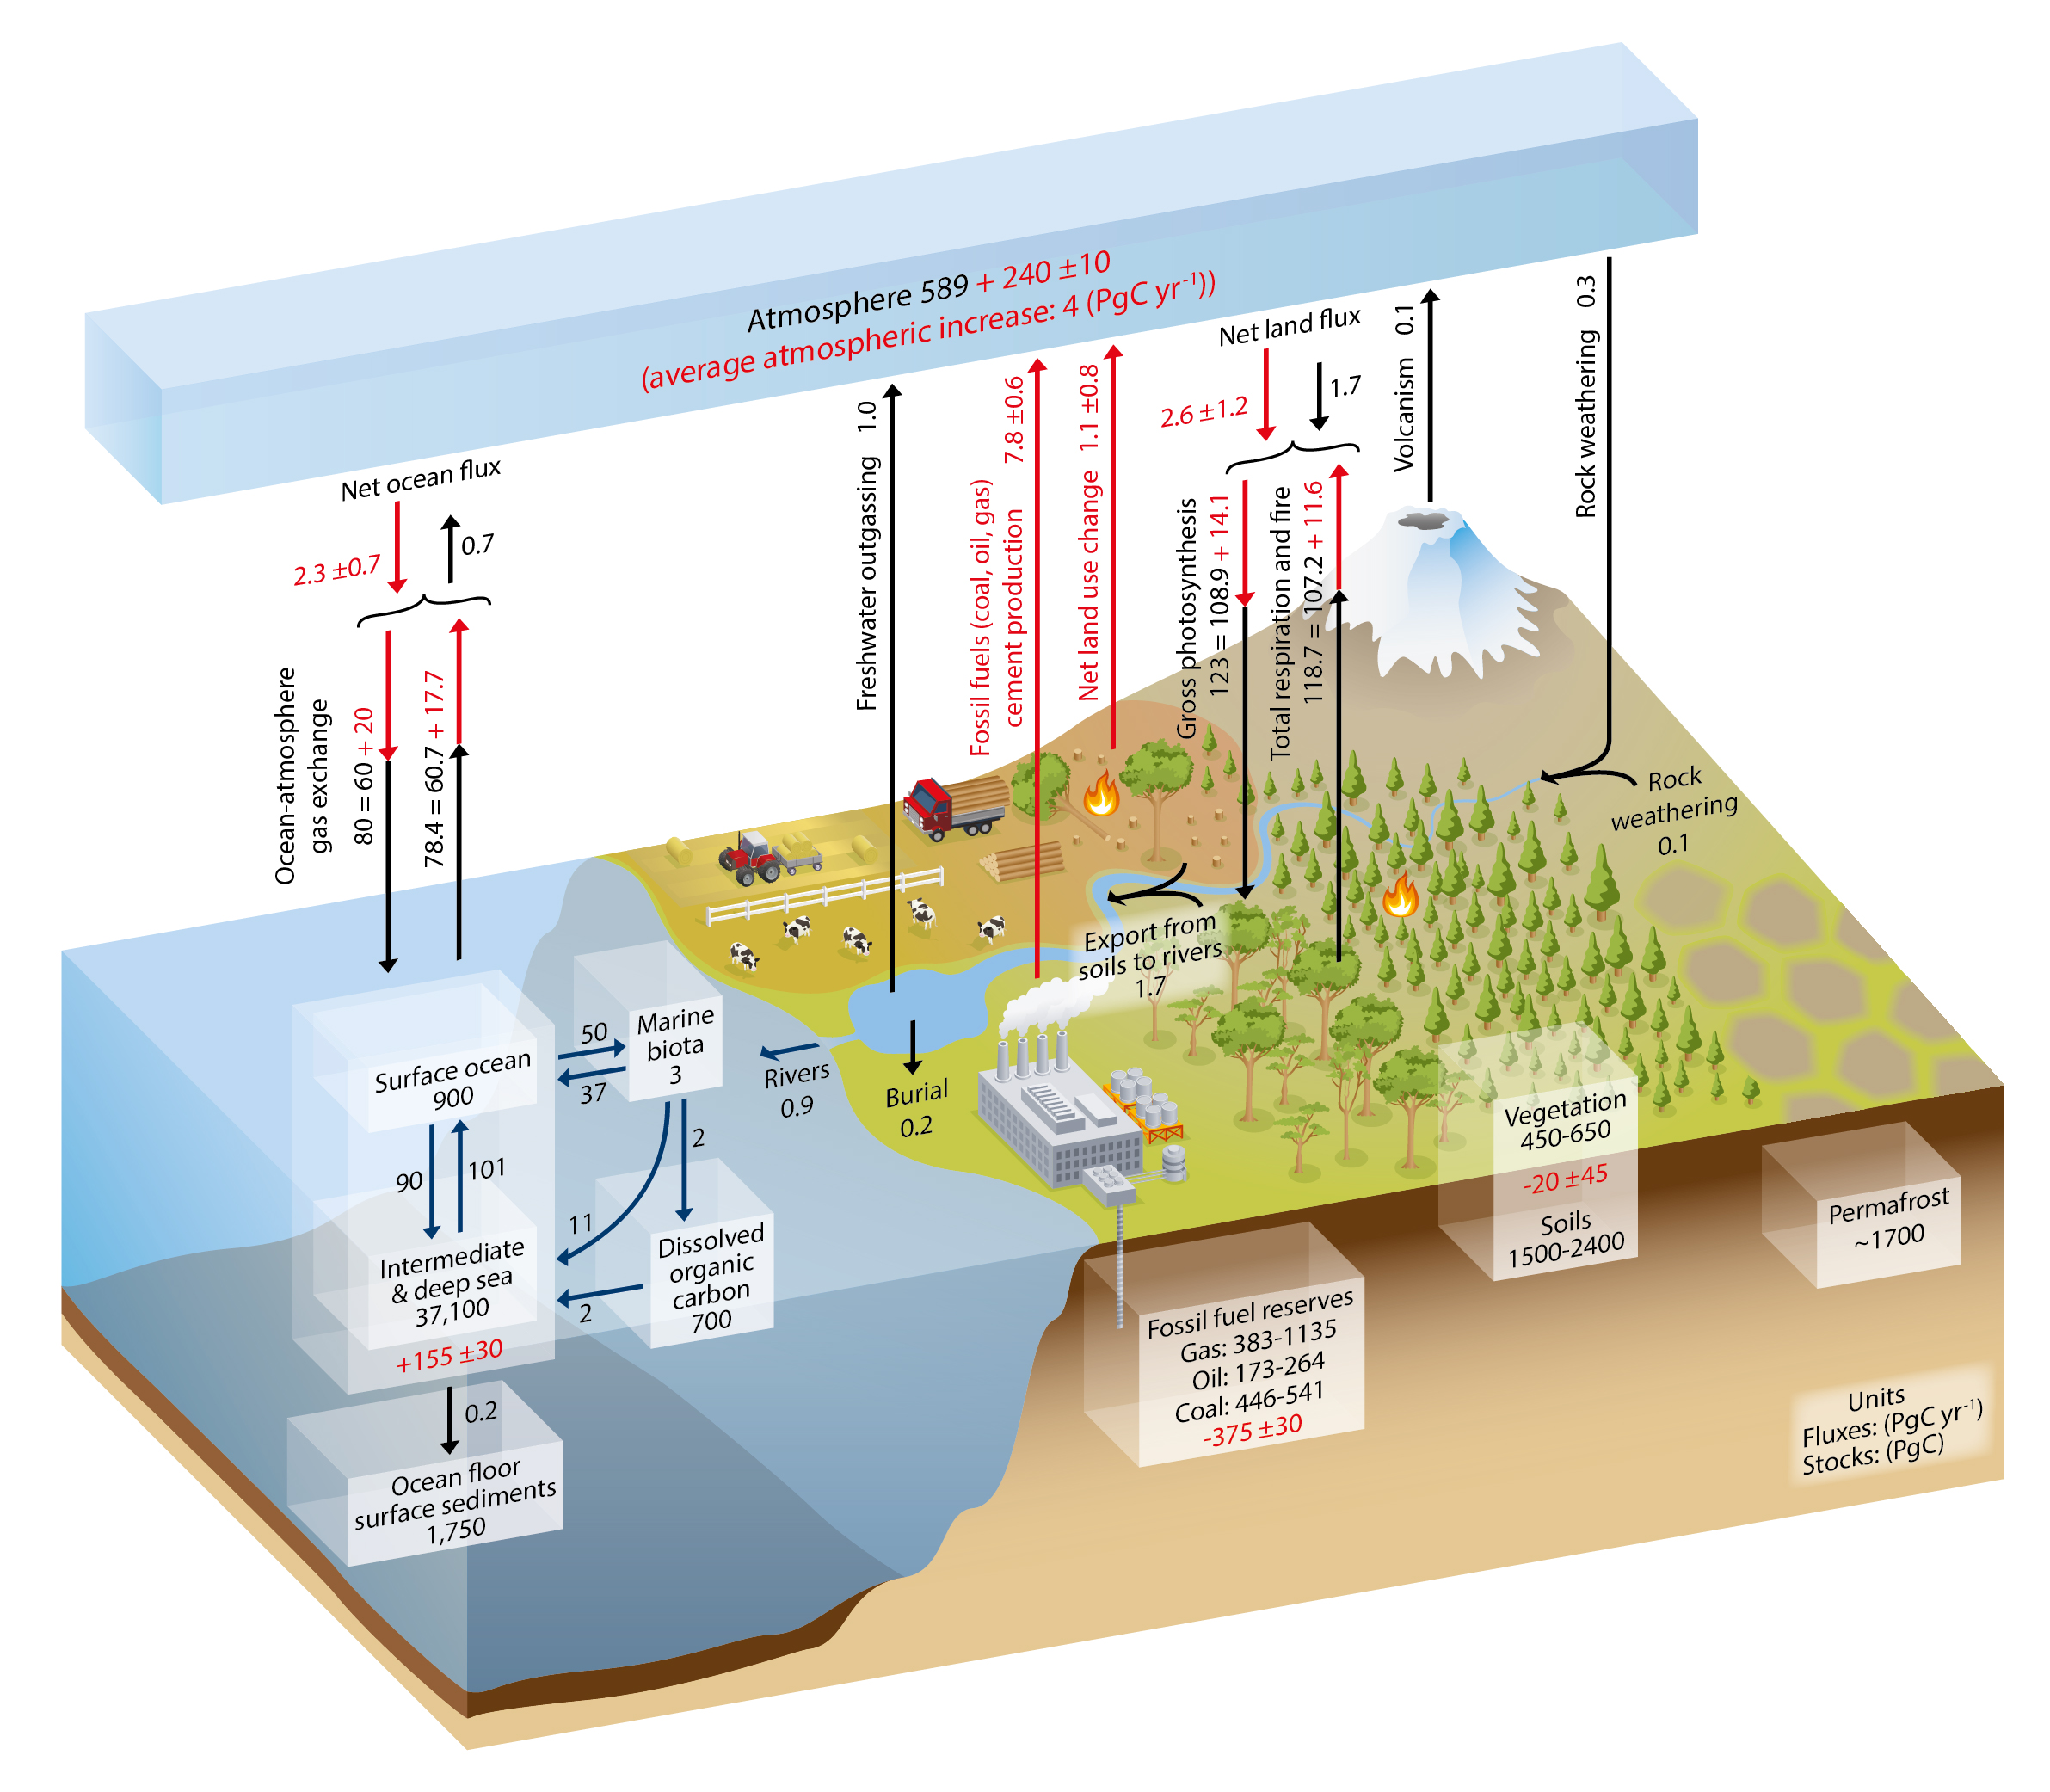
\includegraphics[width=0.7\textwidth]{ipcc_fig6_1.jpg}
    \caption{Global carbon cycle simplified schematic \citep{ciais2014carbon}. Black numbers and arrows represent reservoir mass and exchange fluxes estimated for the time prior to the industrial era (\(\sim\)~1750). Red numbers and arrows represent annual fluxes average over the 2000-2009 time period. Red numbers in the reservoirs indicate the cumulative change of carbon over the industrial period (1750-2011).}
    \label{fig:ipcc_fig6.1}
\end{figure}

IPCC figure 6.1 and 6.8: Partitioning of fluxes important and hard (shown by error on estimates in fig 6.1). Land surface carbon uptake least understood mechanism in the global carbon cycle, ref IPCC. Will uptake remain the same under climate change.

\citet{1748-9326-7-2-024002} Have shown that global warming is highly sensitive to land carbon cycle processes and highlighted the need to improve understanding of land surface carbon uptake and its response to climate change. 

\section{The role of models}

\begin{figure}[ht]
    \centering
    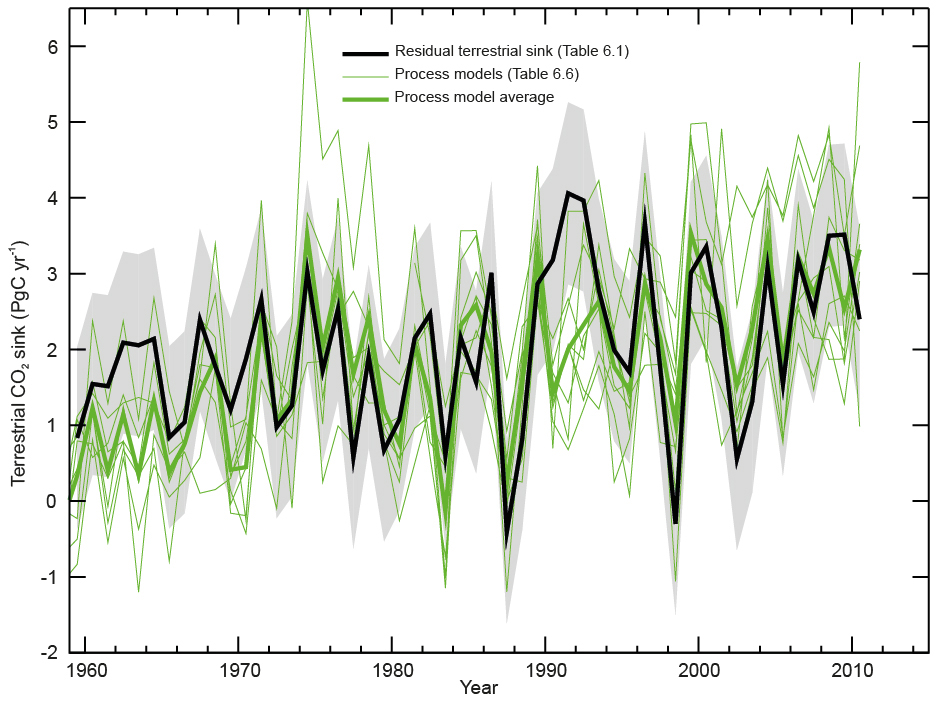
\includegraphics[width=0.9\textwidth]{ipcc_fig6_16.jpg}
    \caption{Modelled land sink \citep{ciais2014carbon}.}
    \label{fig:ipcc_fig6.1}
\end{figure}

IPCC figure 6.16 and section 6.3.2.6.6: Contribution of models to understanding the terrestrial carbon cycle. Reference every DALEC paper.

\section{Eddy covariance and other observations}

Baldocchi paper: Many observations of forest carbon flux made worldwide.

\section{Data assimilation}

Role of DA in NWP improving forecast skill. 


\bibliography{../PhD}{}
\end{document}